\section{Incremental Transformation to Dual}
\label{sect:incremental-transformation-to-dual}

The incremental transformation to dual phase is different from the incremental phase discussed previously in that it doesn't produce yet another sequence of operations. Instead, it takes the sequence of operations produced by the previous phase and applies it directly to the embedded boundary graph produced by the non-incremental transformation or optimization phase in an earlier run through the pipeline. This is also the point in the pipeline where it becomes indispensable that the propagated sequence of operations is tailored towards an already-existing product of the pipeline.

\begin{figure}[H]
	\centering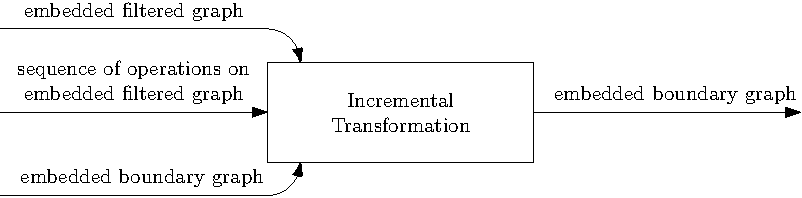
\includegraphics[width=0.9\textwidth]{Resources/DynamicPipeline-IncrementalTransformation.pdf}
	\caption{Input and output of the incremental transformation phase.}
	\label{fig:dynamic-pipeline-incremental-transformation}
\end{figure}

Applying operations for an embedded filtered graph to a boundary graph may appear counter-intuitive or even impossible at first. Keep in mind though that the boundary graph is effectively the dual of the filtered graph and the operations therefore translate 1-to-1 to the boundary graph: operations involving vertices become operations involving faces, edges become face adjacencies, internal faces become points where multiple countries meet, and the outer face becomes the faces that have borders with nothing on the other side. We must therefore be able to make the following changes to an embedded boundary graph:

\begin{itemize}
	\setlength\itemsep{-0.25em}
	\item Insert a region on the inside of the map
	\item Insert a region on the outside of the map
	\item Remove a region on the inside of the map
	\item Remove a region on the outside of the map
	\item Flip a region adjacency on the inside of the map
	\item Create an adjacency between two regions on the outside of the map
	\item Remove an adjacency between two regions on the outside of the map
	\item Update a region's or a region adjacency's weight
\end{itemize}

These changes have the same preconditions as their counterparts on the embedded filtered graph. We will provide visualizations and concrete implementations for making theses in \cref{chap:implementation}.
